\documentclass[a4paper]{article}

%================================================================================================================================
%
% Packages
%
%================================================================================================================================

\usepackage[T1]{fontenc} 	% pour caractères accentués
\usepackage[utf8]{inputenc}  % encodage utf8
\usepackage[french]{babel}	% langue : français
\usepackage{fourier}			% caractères plus lisibles
\usepackage[dvipsnames]{xcolor} % couleurs
\usepackage{fancyhdr}		% réglage header footer
\usepackage{needspace}		% empêcher sauts de page mal placés
\usepackage{graphicx}		% pour inclure des graphiques
\usepackage{enumitem,cprotect}		% personnalise les listes d'items (nécessaire pour ol, al ...)
\usepackage{hyperref}		% Liens hypertexte
\usepackage{pstricks,pst-all,pst-node,pstricks-add,pst-math,pst-plot,pst-tree,pst-eucl} % pstricks
\usepackage[a4paper,includeheadfoot,top=2cm,left=3cm, bottom=2cm,right=3cm]{geometry} % marges etc.
\usepackage{comment}			% commentaires multilignes
\usepackage{amsmath,environ} % maths (matrices, etc.)
\usepackage{amssymb,makeidx}
\usepackage{bm}				% bold maths
\usepackage{tabularx}		% tableaux
\usepackage{colortbl}		% tableaux en couleur
\usepackage{fontawesome}		% Fontawesome
\usepackage{environ}			% environment with command
\usepackage{fp}				% calculs pour ps-tricks
\usepackage{multido}			% pour ps tricks
\usepackage[np]{numprint}	% formattage nombre
\usepackage{tikz,tkz-tab} 			% package principal TikZ
\usepackage{pgfplots}   % axes
\usepackage{mathrsfs}    % cursives
\usepackage{calc}			% calcul taille boites
\usepackage[scaled=0.875]{helvet} % font sans serif
\usepackage{svg} % svg
\usepackage{scrextend} % local margin
\usepackage{scratch} %scratch
\usepackage{multicol} % colonnes
%\usepackage{infix-RPN,pst-func} % formule en notation polanaise inversée
\usepackage{listings}

%================================================================================================================================
%
% Réglages de base
%
%================================================================================================================================

\lstset{
language=Python,   % R code
literate=
{á}{{\'a}}1
{à}{{\`a}}1
{ã}{{\~a}}1
{é}{{\'e}}1
{è}{{\`e}}1
{ê}{{\^e}}1
{í}{{\'i}}1
{ó}{{\'o}}1
{õ}{{\~o}}1
{ú}{{\'u}}1
{ü}{{\"u}}1
{ç}{{\c{c}}}1
{~}{{ }}1
}


\definecolor{codegreen}{rgb}{0,0.6,0}
\definecolor{codegray}{rgb}{0.5,0.5,0.5}
\definecolor{codepurple}{rgb}{0.58,0,0.82}
\definecolor{backcolour}{rgb}{0.95,0.95,0.92}

\lstdefinestyle{mystyle}{
    backgroundcolor=\color{backcolour},   
    commentstyle=\color{codegreen},
    keywordstyle=\color{magenta},
    numberstyle=\tiny\color{codegray},
    stringstyle=\color{codepurple},
    basicstyle=\ttfamily\footnotesize,
    breakatwhitespace=false,         
    breaklines=true,                 
    captionpos=b,                    
    keepspaces=true,                 
    numbers=left,                    
xleftmargin=2em,
framexleftmargin=2em,            
    showspaces=false,                
    showstringspaces=false,
    showtabs=false,                  
    tabsize=2,
    upquote=true
}

\lstset{style=mystyle}


\lstset{style=mystyle}
\newcommand{\imgdir}{C:/laragon/www/newmc/assets/imgsvg/}
\newcommand{\imgsvgdir}{C:/laragon/www/newmc/assets/imgsvg/}

\definecolor{mcgris}{RGB}{220, 220, 220}% ancien~; pour compatibilité
\definecolor{mcbleu}{RGB}{52, 152, 219}
\definecolor{mcvert}{RGB}{125, 194, 70}
\definecolor{mcmauve}{RGB}{154, 0, 215}
\definecolor{mcorange}{RGB}{255, 96, 0}
\definecolor{mcturquoise}{RGB}{0, 153, 153}
\definecolor{mcrouge}{RGB}{255, 0, 0}
\definecolor{mclightvert}{RGB}{205, 234, 190}

\definecolor{gris}{RGB}{220, 220, 220}
\definecolor{bleu}{RGB}{52, 152, 219}
\definecolor{vert}{RGB}{125, 194, 70}
\definecolor{mauve}{RGB}{154, 0, 215}
\definecolor{orange}{RGB}{255, 96, 0}
\definecolor{turquoise}{RGB}{0, 153, 153}
\definecolor{rouge}{RGB}{255, 0, 0}
\definecolor{lightvert}{RGB}{205, 234, 190}
\setitemize[0]{label=\color{lightvert}  $\bullet$}

\pagestyle{fancy}
\renewcommand{\headrulewidth}{0.2pt}
\fancyhead[L]{maths-cours.fr}
\fancyhead[R]{\thepage}
\renewcommand{\footrulewidth}{0.2pt}
\fancyfoot[C]{}

\newcolumntype{C}{>{\centering\arraybackslash}X}
\newcolumntype{s}{>{\hsize=.35\hsize\arraybackslash}X}

\setlength{\parindent}{0pt}		 
\setlength{\parskip}{3mm}
\setlength{\headheight}{1cm}

\def\ebook{ebook}
\def\book{book}
\def\web{web}
\def\type{web}

\newcommand{\vect}[1]{\overrightarrow{\,\mathstrut#1\,}}

\def\Oij{$\left(\text{O}~;~\vect{\imath},~\vect{\jmath}\right)$}
\def\Oijk{$\left(\text{O}~;~\vect{\imath},~\vect{\jmath},~\vect{k}\right)$}
\def\Ouv{$\left(\text{O}~;~\vect{u},~\vect{v}\right)$}

\hypersetup{breaklinks=true, colorlinks = true, linkcolor = OliveGreen, urlcolor = OliveGreen, citecolor = OliveGreen, pdfauthor={Didier BONNEL - https://www.maths-cours.fr} } % supprime les bordures autour des liens

\renewcommand{\arg}[0]{\text{arg}}

\everymath{\displaystyle}

%================================================================================================================================
%
% Macros - Commandes
%
%================================================================================================================================

\newcommand\meta[2]{    			% Utilisé pour créer le post HTML.
	\def\titre{titre}
	\def\url{url}
	\def\arg{#1}
	\ifx\titre\arg
		\newcommand\maintitle{#2}
		\fancyhead[L]{#2}
		{\Large\sffamily \MakeUppercase{#2}}
		\vspace{1mm}\textcolor{mcvert}{\hrule}
	\fi 
	\ifx\url\arg
		\fancyfoot[L]{\href{https://www.maths-cours.fr#2}{\black \footnotesize{https://www.maths-cours.fr#2}}}
	\fi 
}


\newcommand\TitreC[1]{    		% Titre centré
     \needspace{3\baselineskip}
     \begin{center}\textbf{#1}\end{center}
}

\newcommand\newpar{    		% paragraphe
     \par
}

\newcommand\nosp {    		% commande vide (pas d'espace)
}
\newcommand{\id}[1]{} %ignore

\newcommand\boite[2]{				% Boite simple sans titre
	\vspace{5mm}
	\setlength{\fboxrule}{0.2mm}
	\setlength{\fboxsep}{5mm}	
	\fcolorbox{#1}{#1!3}{\makebox[\linewidth-2\fboxrule-2\fboxsep]{
  		\begin{minipage}[t]{\linewidth-2\fboxrule-4\fboxsep}\setlength{\parskip}{3mm}
  			 #2
  		\end{minipage}
	}}
	\vspace{5mm}
}

\newcommand\CBox[4]{				% Boites
	\vspace{5mm}
	\setlength{\fboxrule}{0.2mm}
	\setlength{\fboxsep}{5mm}
	
	\fcolorbox{#1}{#1!3}{\makebox[\linewidth-2\fboxrule-2\fboxsep]{
		\begin{minipage}[t]{1cm}\setlength{\parskip}{3mm}
	  		\textcolor{#1}{\LARGE{#2}}    
 	 	\end{minipage}  
  		\begin{minipage}[t]{\linewidth-2\fboxrule-4\fboxsep}\setlength{\parskip}{3mm}
			\raisebox{1.2mm}{\normalsize\sffamily{\textcolor{#1}{#3}}}						
  			 #4
  		\end{minipage}
	}}
	\vspace{5mm}
}

\newcommand\cadre[3]{				% Boites convertible html
	\par
	\vspace{2mm}
	\setlength{\fboxrule}{0.1mm}
	\setlength{\fboxsep}{5mm}
	\fcolorbox{#1}{white}{\makebox[\linewidth-2\fboxrule-2\fboxsep]{
  		\begin{minipage}[t]{\linewidth-2\fboxrule-4\fboxsep}\setlength{\parskip}{3mm}
			\raisebox{-2.5mm}{\sffamily \small{\textcolor{#1}{\MakeUppercase{#2}}}}		
			\par		
  			 #3
 	 		\end{minipage}
	}}
		\vspace{2mm}
	\par
}

\newcommand\bloc[3]{				% Boites convertible html sans bordure
     \needspace{2\baselineskip}
     {\sffamily \small{\textcolor{#1}{\MakeUppercase{#2}}}}    
		\par		
  			 #3
		\par
}

\newcommand\CHelp[1]{
     \CBox{Plum}{\faInfoCircle}{À RETENIR}{#1}
}

\newcommand\CUp[1]{
     \CBox{NavyBlue}{\faThumbsOUp}{EN PRATIQUE}{#1}
}

\newcommand\CInfo[1]{
     \CBox{Sepia}{\faArrowCircleRight}{REMARQUE}{#1}
}

\newcommand\CRedac[1]{
     \CBox{PineGreen}{\faEdit}{BIEN R\'EDIGER}{#1}
}

\newcommand\CError[1]{
     \CBox{Red}{\faExclamationTriangle}{ATTENTION}{#1}
}

\newcommand\TitreExo[2]{
\needspace{4\baselineskip}
 {\sffamily\large EXERCICE #1\ (\emph{#2 points})}
\vspace{5mm}
}

\newcommand\img[2]{
          \includegraphics[width=#2\paperwidth]{\imgdir#1}
}

\newcommand\imgsvg[2]{
       \begin{center}   \includegraphics[width=#2\paperwidth]{\imgsvgdir#1} \end{center}
}


\newcommand\Lien[2]{
     \href{#1}{#2 \tiny \faExternalLink}
}
\newcommand\mcLien[2]{
     \href{https~://www.maths-cours.fr/#1}{#2 \tiny \faExternalLink}
}

\newcommand{\euro}{\eurologo{}}

%================================================================================================================================
%
% Macros - Environement
%
%================================================================================================================================

\newenvironment{tex}{ %
}
{%
}

\newenvironment{indente}{ %
	\setlength\parindent{10mm}
}

{
	\setlength\parindent{0mm}
}

\newenvironment{corrige}{%
     \needspace{3\baselineskip}
     \medskip
     \textbf{\textsc{Corrigé}}
     \medskip
}
{
}

\newenvironment{extern}{%
     \begin{center}
     }
     {
     \end{center}
}

\NewEnviron{code}{%
	\par
     \boite{gray}{\texttt{%
     \BODY
     }}
     \par
}

\newenvironment{vbloc}{% boite sans cadre empeche saut de page
     \begin{minipage}[t]{\linewidth}
     }
     {
     \end{minipage}
}
\NewEnviron{h2}{%
    \needspace{3\baselineskip}
    \vspace{0.6cm}
	\noindent \MakeUppercase{\sffamily \large \BODY}
	\vspace{1mm}\textcolor{mcgris}{\hrule}\vspace{0.4cm}
	\par
}{}

\NewEnviron{h3}{%
    \needspace{3\baselineskip}
	\vspace{5mm}
	\textsc{\BODY}
	\par
}

\NewEnviron{margeneg}{ %
\begin{addmargin}[-1cm]{0cm}
\BODY
\end{addmargin}
}

\NewEnviron{html}{%
}

\begin{document}
\meta{url}{/exercices/fonction-exponentielle-bac-blanc-es-l-sujet-3-maths-cours-2018/}
\meta{pid}{10475}
\meta{titre}{Fonction exponentielle - Bac blanc ES/L Sujet 3 - Maths-cours 2018}
\meta{type}{exercices}
%
\begin{h2}Exercice 3 (5 points)\end{h2}
\par
On a représenté, ci-après, la courbe $\mathscr{C}$ d'une fonction définie et dérivable sur l'intervalle $[0~;~5]$ ainsi que la tangente $T$ à cette courbe au point $O$, origine du repère.
\par
\begin{center}
     \begin{extern}%width="550" alt="Courbe représentative de f"
          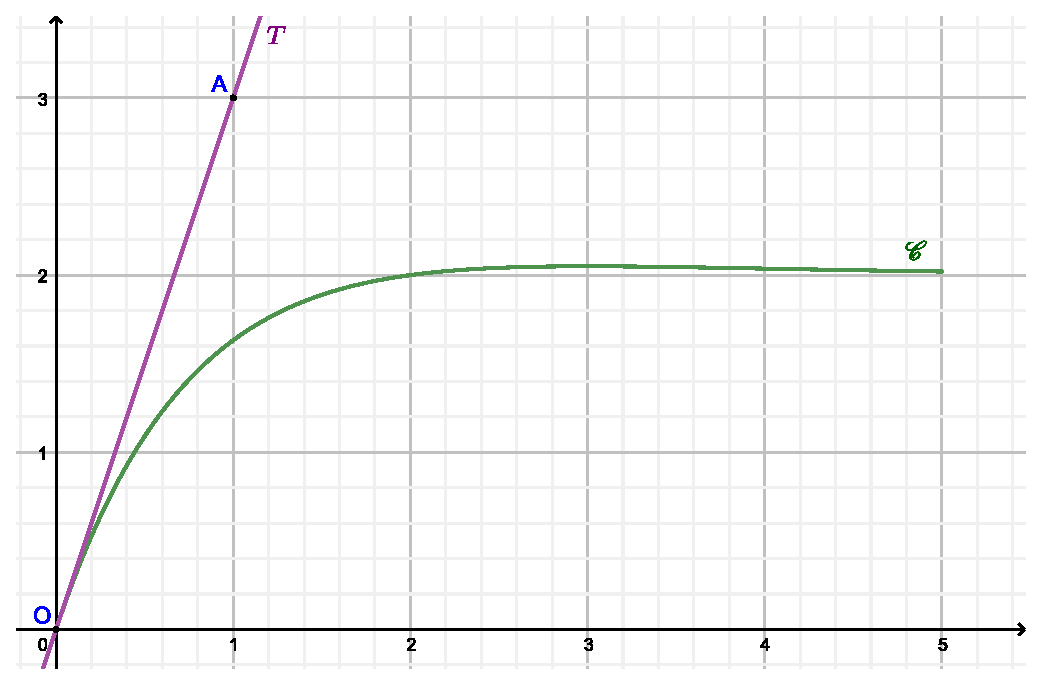
\includegraphics[width=0.9\textwidth]{images/BBESL-s3-3-1}% gbb 1 unite=3cm
     \end{extern}
\end{center}
\begin{center}
\imgsvg{BBESL-s3-3-1}{0.3}% alt="Construction des termes d'une suite récurrente " style="width:50rem"
\end{center}
\par
On note $f'$ la fonction dérivée de la fonction $f$.
\par
%============================================================================================================================
%
\TitreC{Partie A}
%
%============================================================================================================================
\par
\begin{enumerate}
     \item
     Préciser la valeur de $f(0)$.
     \item
     La tangente $T$ passe par le point $A(1~;~3)$.
     \par
     Déterminer la valeur de $f'(0)$.
     \item
     On admet que la fonction $f$ est définie sur l'intervalle $[0~;~5]$ par une expression de la forme :
     \[ f(x)=(ax+b)\text{e}^{-x}+2 \]
     \par
     où $a$ et $b$ sont deux nombres réels.
     \par
     \begin{enumerate}
          \item
          Montrer que pour tout réel $x$ de l'intervalle $[0~;~5]$ :
          \[ f'(x)=(-ax+a-b)\text{e}^{-x}. \]
          \item
          \`A l'aide des questions \textbf{1.} et \textbf{2.}, déterminer les valeurs de $a$ et $b$.
          \par
     \end{enumerate}
     \par
\end{enumerate}
\par
%============================================================================================================================
%
\TitreC{Partie B}
%
\par
Par la suite, on considèrera que la fonction $f$ est définie sur l'intervalle $[0~;~5]$ par :
\[ f(x)=(x-2)\text{e}^{-x}+2. \]
\par
\begin{enumerate}
     \item
     Calculer $f'(x)$ et tracer le tableau de variations de $f$ sur l'intervalle $[0~;~5]$.
     \par
     On placera, dans le tableau, les valeurs exactes de $f(0)$, de $f(5)$ et du maximum de $f$ sur l'intervalle $[0~;~5]$.
     \item
     Montrer que l'équation $f(x)=1$ admet une unique solution $\alpha$ sur l'intervalle $[0~;~5]$.
     \item
     Donner un encadrement de $\alpha$ d'amplitude $10^{-3}$.
     \item
     Montrer que la courbe $\mathscr{C}$ possède un unique point d'inflexion dont on déterminera les coordonnées.
     \par
\end{enumerate}
\begin{corrige}
     %============================================================================================================================
     %
     \TitreC{Partie A}
     %
     %============================================================================================================================
     \par
     \begin{enumerate}
          \item %1
          La courbe $\mathscr{C}$ passe par le point $O(0~;~0)$. Par conséquent :
          \[ f(0)=0. \]
          \item %2
          $f'(0)$ est le coefficient directeur de la tangente $T$ au point $O$. Cette droite passe par les points $O(0~;~0)$ et $A(1~;~3)$ donc :
          \par
          $f'(0)=\dfrac{y_A-y_O}{x_A-x_0}=\dfrac{3-0}{1-0}=3$.
          \item %3
          \begin{enumerate}
               \item %3a
               La fonction $f$ est définie et dérivable sur l'intervalle $[0~;~5]$ et ${f(x)=(ax+b)\text{e}^{-x}+2}$.
               \par
               Posons $u(x)=ax+b$ et $v(x)=\text{e}^{-x}$.
               \par
               Alors :
               \par
               $u'(x)=a$ et $v'(x)=-\text{e}^{-x}$.
               \par
               Par ailleurs, 2 étant une constante, la dérivée de la fonction ${x \longmapsto 2}$ est nulle ; par conséquent :
               \par
               $f'(x)=u'(x)v(x)+u(x)v'(x)$
               \par
               $\phantom{f'(x)}=a \text{e}^{-x}+(ax+b)(-\text{e}^{-x})$
               \par
               $\phantom{f'(x)}=a \text{e}^{-x}-(ax+b)\text{e}^{-x}$
               \par
               $\phantom{f'(x)}=a \text{e}^{-x}-ax\text{e}^{-x} - b\text{e}^{-x}$.
               \par
               On factorise $\text{e}^{-x}$ :
               \par
               $f'(x)=(-ax+a-b)\text{e}^{-x}$.
               \par
               \cadre{rouge}{Attention}{
                    La dérivée du produit $uv$ n'est pas $u'v'$ mais $u'v+uv'$ !
               }
               \item %3b
               Comme $f(x)=(ax+b)\text{e}^{-x}+2$, alors :
               \par
               $f(0)=b\text{e}^{0}+2=b+2$.
               \par
               Par ailleurs, $f'(x)=(-ax+a-b)\text{e}^{-x}$ donc :
               \par
               $f'(0)=(a-b)\text{e}^{0}=a-b$.
               \par
               Or, $f(0)=0$ donc $b+2=0$ et $b=-2$.
               \par
               De plus $f'(0)=3$ donc $a-b=3$ soit ${a=b+3=-2+3=1}$.
               \par
               \cadre{vert}{En pratique}{
                    Pour déterminer $a$ et $b$, \textbf{pensez à utiliser les résultats des questions précédentes} (ici, c'est même indiqué dans l'énoncé !).
                    \par
                    Les égalités $f(0)=0$ et $f'(0)=3$ nous donnent deux équations qui nous permettent de déterminer $a$ et $b$.
               }
               \par
               $f$ est donc définie sur $[0~;~5]$ par :
               \[ f(x)=(x-2)\text{e}^{-x}+2. \]
               \par
          \end{enumerate}
          \par
     \end{enumerate}
     \par
     %============================================================================================================================
     %
     \TitreC{Partie B}
     %
     %============================================================================================================================
     \par
     \begin{enumerate}
          \item %1
          La fonction $f : x \longmapsto (x-2)\text{e}^{-x}+2$ est définie et dérivable sur l'intervalle $[0~;~5]$.
          \par
          Posons $u(x)=x-2$ et $v(x)=\text{e}^{-x}$.
          \par
          Alors :
          \par
          $u'(x)=1$ et $v'(x)=-\text{e}^{-x}$.
          \par
          $f'(x)=u'(x)v(x)+u(x)v'(x) + 0$
          \par
          $\phantom{f'(x)}= \text{e}^{-x}+(x-2)(-\text{e}^{-x})$
          \par
          $\phantom{f'(x)}= \text{e}^{-x}-(x-2)\text{e}^{-x}$
          \par
          $\phantom{f'(x)}= \text{e}^{-x}-x\text{e}^{-x} + 2\text{e}^{-x}$.
          \par
          On factorise $\text{e}^{-x}$ :
          \par
          $f'(x)=(3-x)\text{e}^{-x}$.
          \par
          \cadre{bleu}{Remarque}{
               Pour calculer $f'(x)$ on pouvait également utiliser le résultat de la question \textbf{3.a.} et remplacer $a$ par $1$ et $b$ par $-2$.
          }
          \par
          La fonction exponentielle prend ses valeurs dans l'intervalle $]0~;+~\infty[$ donc, pour tout réel $x$, ${\text{e}^{-x} > 0}$.
          \par
          $f'(x)$ est donc du signe de $3-x$.
          \par
          La fonction $x \longmapsto 3-x$ est une fonction affine qui s'annule pour $x=3$ et est strictement positive si et seulement si $x < 3$.
          \par
          De plus :
          \par
          $f(3)=(3-2)\text{e}^{-3}+2=\text{e}^{-3}+2\ $ et $f(5)=(5-2)\text{e}^{-5}+2=3\text{e}^{-5}+2$.
          \par
          On en déduit le tableau de variations de $f$ :
          \par
          %:-+-+-+-+- Engendré par : http://math.et.info.free.fr/TikZ/TableauxVariations/
          \begin{center}
               \begin{extern}%width="360" alt="Tableau de variations de f"
                    \begin{tikzpicture}[scale=0.875]
                         % Styles
                         \tikzstyle{cadre}=[thin]
                         \tikzstyle{fleche}=[->,>=latex,thin]
                         \tikzstyle{nondefini}=[lightgray]
                         % Dimensions Modifiables
                         \def\Lrg{1.5}
                         \def\HtX{1}
                         \def\HtY{0.5}
                         % Dimensions Calculées
                         \def\lignex{-0.5*\HtX}
                         \def\lignef{-1.5*\HtX}
                         \def\separateur{-0.5*\Lrg}
                         % Largeur du tableau
                         \def\gauche{-1.5*\Lrg}
                         \def\droite{4.6*\Lrg}
                         % Hauteur du tableau
                         \def\haut{0.5*\HtX}
                         \def\bas{-2.5*\HtX-2*\HtY}
                         % Ligne de l'abscisse : x
                         \node at (-1*\Lrg,0) {$x$};
                         \node at (0*\Lrg,0) {$0$};
                         \node at (2*\Lrg,0) {$3$};
                         \node at (4*\Lrg,0) {$5$};
                         % Ligne de la dérivée : f'(x)
                         \node at (-1*\Lrg,-1*\HtX) {$f'(x)$};
                         \node at (0*\Lrg,-1*\HtX) {$\ $};
                         \node at (1*\Lrg,-1*\HtX) {$+$};
                         \node at (2*\Lrg,-1*\HtX) {$0$};
                         \node at (3*\Lrg,-1*\HtX) {$-$};
                         \node at (4*\Lrg,-1*\HtX) {$\ $};
                         % Ligne de la fonction : f(x)
                         \node  at (-1*\Lrg,{-2*\HtX+(-1)*\HtY}) {$f(x)$};
                         \node (f1) at (0*\Lrg,{-2*\HtX+(-2)*\HtY}) {$0$};
                         \node (f2) at (2*\Lrg,{-2*\HtX+(0)*\HtY}) {$\text{e}^{-3}+2$};
                         \node (f3) at (3.9*\Lrg,{-2*\HtX+(-2)*\HtY}) {$3\text{e}^{-5}+2$};
                         % Flèches
                         \draw[fleche] (f1) -- (f2);
                         \draw[fleche] (f2) -- (f3);
                         % Encadrement
                         \draw[cadre] (\separateur,\haut) -- (\separateur,\bas);
                         \draw[cadre] (\gauche,\haut) rectangle  (\droite,\bas);
                         \draw[cadre] (\gauche,\lignex) -- (\droite,\lignex);
                         \draw[cadre] (\gauche,\lignef) -- (\droite,\lignef);
                    \end{tikzpicture}
               \end{extern}
          \end{center}
          \cadre{bleu}{Remarque}{
               Sauf indication contraire de l'énoncé, il est préférable de \textbf{conserver les valeurs exactes} (ici, c'est même impératif car précisé dans la question) dans le tableau de variations, quitte à calculer une valeur approchée par la suite si nécessaire.
          }
          \item %2
          $\text{e}^{-3}+2 \approx 2,05$\\
          $3\text{e}^{-5}+2 \approx 2,02$
          \par
          Sur l'intervalle $[0~;~3]$, $f$ est \textbf{continue} et \textbf{strictement croissante}. 1 appartient à l'intervalle $[0~;\text{e}^{-3}+2 ]$ donc l'équation $f(x)=1$ admet une unique solution sur l'intervalle $[0~;~3]$.
          \par
          Sur l'intervalle $[3~;~5]$, le minimum de $f$ est supérieur à 2 donc l'équation ${f(x)=1}$ n'a pas de solution sur cet intervalle.
          \par
          Par conséquent, l'équation $f(x)=1$ admet une unique solution sur l'intervalle $[0~;~5]$.
          \item %3
          \`A la calculatrice \textit{(voir détails  \hyperlink{tvi-pap}{ci-après})}, on trouve :
          \par
          $f(0,442) \approx 0,9986 < 1$ ;
          \par
          $f(0,443) \approx 1,0002 > 1$.
          \par
          Par conséquent : $0,442 < \alpha < 0,443$.
          \par
          \cadre{rouge}{Bien rédiger}{
               Pour justifier un encadrement du type ${\alpha_1 < \alpha < \alpha_2}$, vous pouvez indiquer sur votre copie les valeurs de $f(\alpha_1)$ et de $f(\alpha_2)$ que vous avez obtenues à la calculatrice.
          }
          \item %4
          La fonction $f' : x \longmapsto (3-x)\text{e}^{-x}$ est dérivable sur l'intervalle $[0~;~5]$.
          \par
          Posons $u(x)=3-x$ et $v(x)=\text{e}^{-x}$.
          \par
          Alors :
          \par
          $u'(x)=-1$ et $v'(x)=-\text{e}^{-x}$.
          \par
          $f''(x)=u'(x)v(x)+u(x)v'(x) + 0$
          \par
          $\phantom{f''(x)}= -1 \times \text{e}^{-x}+(3-x)(-\text{e}^{-x})$
          \par
          $\phantom{f''(x)}= -\text{e}^{-x}-(3-x)\text{e}^{-x}$
          \par
          $\phantom{f''(x)}=(-1-3+x)\text{e}^{-x}$
          \par
          $\phantom{f''(x)}=(x-4)\text{e}^{-x}$.
          \par
          Pour tout réel $x$, ${\text{e}^{-x} > 0}$, donc $f''(x)$ est donc du signe de $x-4$.
          \par
          La fonction $x \longmapsto x-4$ est une fonction affine qui s'annule pour et \textbf{change de signe} pour $x=4$.
          \par
          La courbe $\mathscr{C}$ possède donc un unique point d'inflexion d'abscisse $4$ et d'ordonnée $f(4)=2 \text{e}^{-4}+2$.
          \par
     \end{enumerate}
\end{corrige}

\end{document}